% Created 2020-11-18 Wed 13:52
% Intended LaTeX compiler: xelatex
\documentclass[xcolor=table,10pt,aspectratio=169]{beamer}
\RequirePackage{etex}
\RequirePackage[l2tabu,orthodox]{nag}            %% Warn about obsolete commands and packages
\RequirePackage{amsmath,amsfonts,amssymb,amsthm} %% Math
\RequirePackage{ifxetex,ifluatex}                %% Detect XeTeX and LuaTeX
\RequirePackage{fixltx2e}                        %% provides \textsubscript
\RequirePackage{xspace}
\RequirePackage{graphicx}
\RequirePackage{comment}
\RequirePackage{url}
\RequirePackage{relsize}
\RequirePackage{booktabs}
\RequirePackage{tabularx}
\RequirePackage[normalem]{ulem}
\RequirePackage[all]{xy}
\RequirePackage{etoolbox}

%%%
%%% Code Listings
%%%

\RequirePackage{listings}
\lstdefinelanguage{Sage}[]{Python}{morekeywords={True,False,sage,cdef,cpdef,ctypedef,self},sensitive=true}

\lstset{frame=none,
  showtabs=False,
  showspaces=False,
  showstringspaces=False,
  commentstyle={\color{gray}},
  keywordstyle={\color{mLightBrown}\textbf},
  stringstyle ={\color{mDarkBrown}},
  frame=single,
  basicstyle=\tt\scriptsize\relax,
  backgroundcolor=\color{gray!190!black},
  inputencoding=utf8,
  literate={…}{{\ldots}}1,
  belowskip=0.0em,
}

\makeatletter
\patchcmd{\@verbatim}
  {\verbatim@font}
  {\verbatim@font\scriptsize}
  {}{}
\makeatother

%%%
%%% Tikz
%%%

\RequirePackage{tikz,pgfplots}
\pgfplotsset{compat=newest}

\usetikzlibrary{calc}
\usetikzlibrary{arrows}
\usetikzlibrary{automata}
\usetikzlibrary{positioning}
\usetikzlibrary{decorations.pathmorphing}
\usetikzlibrary{backgrounds}
\usetikzlibrary{fit,}
\usetikzlibrary{shapes.symbols}
\usetikzlibrary{chains}
\usetikzlibrary{shapes.geometric}
\usetikzlibrary{shapes.arrows}
\usetikzlibrary{graphs}

%% Cache but disable by default

\usetikzlibrary{external}
\tikzexternalize[]
\tikzset{external/export=false}

%%%
%%% SVG (Inkscape)
%%%

\ifxetex % chktex 1
\providecommand{\executeiffilenewer}[3]{%
  {\immediate\write18{#3}} % hack
}
\else
\providecommand{\executeiffilenewer}[3]{%
  \ifnum\pdfstrcmp{\pdffilemoddate{#1}}%
    {\pdffilemoddate{#2}}>0%
    {\immediate\write18{#3}}
  \fi%
}
\fi

\providecommand{\includesvg}[2][1.0\textwidth]{%
 \executeiffilenewer{#1.svg}{#1.pdf}%
 {inkscape -z -D --file=#2.svg --export-pdf=#2.pdf --export-latex --export-area-page}%
 \def\svgwidth{#1} 
 \input{#2.pdf_tex}%
} 

%%%
%%% Metropolis Theme
%%%

\usetheme{metropolis}
\metroset{color/block=fill}
\metroset{numbering=none}
\metroset{outer/progressbar=foot}
\metroset{titleformat=smallcaps}

\setbeamercolor{description item}{fg=mLightBrown}
% \setbeamerfont{alerted text}{series=\bfseries}
\setbeamerfont{footnote}{size=\scriptsize}
\setbeamercolor{example text}{fg=mDarkBrown}
\setbeamercolor{block title alerted}{fg=white, bg=mDarkBrown}
\setbeamertemplate{bibliography item}[text]

\renewcommand*{\UrlFont}{\ttfamily\relax}

%%%
%%% UTF-8 & Fonts
%%% 

\RequirePackage{unicodesymbols} % after metropolis which loads fontspec

\setmonofont[BoldFont={Cousine Bold},
             ItalicFont={Cousine Italic},
             BoldItalicFont={Cousine Bold Italic},
             Scale=0.9]{Cousine}             
%%%
%%% BibLaTeX
%%%

\RequirePackage[backend=bibtex,
            style=alphabetic,
            maxnames=4,
            citestyle=alphabetic]{biblatex}

\bibliography{local.bib,abbrev3.bib,crypto_crossref.bib,rfc.bib,jacm.bib,dcc.bib}

\DeclareFieldFormat{title}{\alert{#1}}
\DeclareFieldFormat[book]{title}{\alert{#1}}
\DeclareFieldFormat[thesis]{title}{\alert{#1}}
\DeclareFieldFormat[inproceedings]{title}{\alert{#1}}
\DeclareFieldFormat[incollection]{title}{\alert{#1}}
\DeclareFieldFormat[article]{title}{\alert{#1}}
\DeclareFieldFormat[misc]{title}{\alert{#1}}

%%% 
%%% Microtype
%%%

\IfFileExists{upquote.sty}{\RequirePackage{upquote}}{}
\IfFileExists{microtype.sty}{\RequirePackage{microtype}}{}

\setlength{\parindent}{0pt}                   %%
\setlength{\parskip}{6pt plus 2pt minus 1pt}  %%
\setlength{\emergencystretch}{3em}            %% prevent overfull lines
\setcounter{secnumdepth}{0}                   %%

%%% Local Variables:
%%% mode: latex
%%% End:
\usepackage{graphicx}
\usepackage{grffile}
\usepackage{longtable}
\usepackage{wrapfig}
\usepackage{rotating}
\usepackage[normalem]{ulem}
\usepackage{amsmath}
\usepackage{textcomp}
\usepackage{amssymb}
\usepackage{capt-of}
\usepackage{hyperref}
\usepackage{microtype}
\usepackage{newunicodechar}
\usepackage[notions,operators,sets,keys,ff,adversary,primitives,complexity,asymptotics,lambda,landau,advantage]{cryptocode}
\usepackage{xspace}
\usepackage{units}
\usepackage{nicefrac}
\usepackage{gensymb}
\usepackage{amsthm}
\usepackage{amsmath}
\usepackage{amssymb}
\usepackage{xcolor}
\usepackage{listings}
\usepackage[color=yellow!40]{todonotes}
\newcommand{\Ldis}{\ensuremath{\mathcal{L}_{\mathbf{s},\chi}}\xspace}
\newcommand{\rhf}{{\ensuremath{\sqrt{\alpha_{\beta}}}\xspace}}
\DeclareMathOperator{\Vol}{Vol}
\renewcommand{\vec}[1]{\ensuremath{\mathbf{#1}}\xspace}
\renewcommand{\norm}[1]{\left\lVert#1\right\rVert}
\newcommand{\mat}[1]{\ensuremath{\vec{#1}}\xspace}
\usetheme{default}
\author{Martin R. Albrecht}
\date{18 November 2020}
\title{LWE and Encryption}
\subtitle{Indian Workshop on Post-Quantum Cryptography}
\hypersetup{
pdfauthor={Martin R. Albrecht},
pdftitle={LWE and Encryption},
pdfkeywords={},
pdfsubject={},
pdfcreator={Emacs 28.0.50 (Org mode 9.4)},
pdflang={English},
colorlinks,
citecolor=gray,
filecolor=gray,
linkcolor=gray,
urlcolor=gray
}
\begin{document}

\maketitle
\begin{frame}{Outline}
\tableofcontents
\end{frame}


\section{LWE}
\label{sec:org3c54f9e}

\begin{frame}[label={sec:orga1297bc}]{1-dim LWE (even easier than RSA)}
\begin{columns}[t]
\begin{column}{0.4\columnwidth}
\textbf{KeyGen}

\begin{itemize}
\item Pick an integer \(q \approx 2^{10000}\)
\item Pick a random integer \(s \in \ZZ_q\)
\item Pick about \(t=20000\) random \(a_i \in \ZZ_q\) and \(e_i \approx 2^{9990}\)
\item Publish pairs \(a_i, c_i = a_i \cdot s + e_i \bmod \ZZ_q\)
\end{itemize}

\textbf{Encrypt}  \(m \in \{0,1\}\)

\begin{itemize}
\item Pick \(b_i \in \{-1,0,1\}\)
\item \(d_0 = \sum_{i=0}^{t-1} b_i \cdot a_i\)
\item \(d_1 = q/2\cdot m + \sum_{i=0}^{t-1} b_i \cdot c_i\)
\item Return \(d_0, d_1\)
\end{itemize}
\end{column}

\begin{column}{0.6\columnwidth}
\textbf{Decrypt}

\begin{itemize}
\item Compute \(d = d_1 - d_0 \cdot s\)
\begin{align*}
  &= q/2\cdot m + \sum_{i=0}^{t-1} b_i \cdot c_i - \sum_{i=0}^{t-1} b_i \cdot a_i \cdot s\\
  &= q/2\cdot m + \sum_{i=0}^{t-1} b_i \cdot (a_i \cdot s + e_i) - \sum_{i=0}^{t-1} b_i \cdot a_i \cdot s\\
  &= q/2\cdot m + \sum_{i=0}^{t-1} b_i \cdot  e_i 
\end{align*}
\item Return 1 if \(d\) is closer to \(q/2\) than zero and 0 otherwise.
\end{itemize}
\end{column}
\end{columns}
\end{frame}

\begin{frame}[label={sec:orgd6cb48a}]{The Learning with Errors Problem (LWE)}
Given \((\vec{A},\vec{c})\) with \(\vec{c} \in \ZZ_q^{m}\), \(\vec{A} \in \ZZ_q^{m \times n}\), \(\vec{s} \in \ZZ_q^{n}\) and \alert{small \(\vec{e} \in \ZZ^{m}\)} is

\begin{align*}
\left(\begin{array}{c}
\\
\\
\\ 
\vec{c} \\
\\
\\
\\
\end{array} \right) = \left(
\begin{array}{ccc}
\leftarrow & n & \rightarrow \\
\\
\\ 
& \vec{A} & \\
\\
\\
\\
\end{array} \right) \times \left( \begin{array}{c}
\\
\vec{s} \\
\\
\end{array} \right) \alert{+ \left(
\begin{array}{c}
\\
\\
\\ 
\vec{e} \\
\\
\\
\\
\end{array} 
\right)}
\end{align*}

or \(\vec{c} \sample \mathcal{U}\left(\ZZ_q^{m}\right)\).
\end{frame}

\begin{frame}[label={sec:orge1a672a}]{The Learning with Errors Problem (LWE)}
\begin{definition}
Let \(n,\,q\) be positive integers, \(\chi\) be a probability distribution on \(\ZZ\) and \(\vec{s}\) be a uniformly random vector in \(\ZZ_q^n\). We denote by \(\Ldis\) the probability distribution on \(\ZZ_q^n \times \ZZ_q\) obtained by choosing \(\vec{a} \in \ZZ_q^n\) uniformly at random, choosing \(e \in \ZZ\) according to \(\chi\) and considering it in \(\ZZ_q\), and returning  \((\vec{a},c) = (\vec{a},\langle \vec{a},\vec{s} \rangle+ e) \in \ZZ_q^n \times \ZZ_q\).

\begin{description}
\item[{Decision-LWE}] is the problem of deciding whether pairs \((\vec{a}, c) \in \ZZ_q^n \times \ZZ_q\) are sampled according to \(\Ldis\) or the uniform distribution on \(\ZZ_q^n \times \ZZ_q\).

\item[{Search-LWE}] is the problem of recovering \(\vec{s}\) from pairs \((\vec{a}, c)=(\vec{a},\langle  \vec{a},\vec{s}\rangle + e) \in \ZZ_q^n \times \ZZ_q\) sampled according to \(\Ldis\).
\end{description}
\end{definition}

\fullcite{Regev:2009:LLE}
\end{frame}

\begin{frame}[label={sec:orgc0c94a2}]{A Fair Warning}
\begin{alertblock}{Gaussian Distributions}
In this talk I am ignoring the specifics of the distribution \(\chi\). That is, the only slide with the phrase "Discrete Gaussian distribution" is this slide.

In practice, \textbf{for encryption} the shape of the error does not seem to matter much.

Also, ignoring the distribution allows to brutally simply proof sketches: almost all technical difficulty in these proofs derives from arguing about two distributions being close.
\end{alertblock}
\end{frame}

\begin{frame}[label={sec:org2d8be9b}]{Normal Form LWE}
\begin{itemize}
\item Consider \(\mat{A} \in \ZZ_q^{2n \times n}\), with \(\mat{A}^T = \left[\mat{A}_0^T \mid \mat{A}_1^T\right]\), \(\vec{s} \in \ZZ_q^n\), \(\vec{e} \sample \chi^m\) with \(\vec{e}^T = \left(\vec{e}_0^T \mid \vec{e}_1^T\right)\)

\item We have \(\vec{c}_0 = \mat{A}_0 \cdot \vec{s} + \vec{e}_0\) and \(\vec{c}_1 = \vec{A}_1 \cdot \vec{s} + \vec{e}_1\)

\item We also have
\begin{align*}
\vec{c}' &= \vec{c}_1 - \mat{A}_1 \cdot \mat{A}_0^{-1} \cdot \vec{c}_0\\
   &= \vec{A}_1\cdot \vec{s} + \vec{e}_1 -  \mat{A}_1 \cdot \mat{A}_0^{-1} (\mat{A}_0 \cdot \vec{s} + \vec{e}_0)\\
   &= \vec{A}_1\cdot \vec{s} + \vec{e}_1 -  \mat{A}_1 \cdot \vec{s} -  \mat{A}_1 \cdot \mat{A}_0^{-1} \cdot \vec{e}_0\\
   &= - \mat{A}_1 \cdot \mat{A}_0^{-1} \cdot \vec{e}_0 + \vec{e}_1\\
   &= \mat{A}' \cdot \vec{e}_0 + \vec{e}_1
\end{align*}
\end{itemize}

\begin{block}{\cite{C:ACPS09}}
We might as well assume that our secret is also sampled from \(\chi\).
\end{block}
\end{frame}

\begin{frame}[label={sec:org93d4f7b}]{Dimension/Modulus Trade-Off}
Consider \(\vec{a}, \vec{s} \in \mathbb{Z}_{q}^{d}\) where \(\vec{s}\) is small, then
\[q^{d-1} \cdot \langle{\vec{a},\vec{s}}\rangle \approx \left(\sum_{i=0}^{d-1} q^{i} \cdot a_{i}\right) \cdot \left(\sum_{i=0}^{d-1} q^{d-i-1} \cdot s_{i}\right) \bmod q^{d} = \tilde{a} \cdot \tilde{s} \bmod q^{d}.\]
Thus, if there exists an efficient algorithm solving the problem in \(\ZZ_{q^d}\), we can use it to solve the problem in \(\mathbb{Z}_{q}^d\). 

\begin{example}[\(\ZZ_{q^{2}}\)]
\[q\cdot \left(a_{0}\cdot s_{0} + a_{1} \cdot s_{1}\right) + a_{0} \cdot s_{1} + q^{2} \cdot a_{1} \cdot s_{0} \bmod q = \left(a_{0} + q\cdot a_{1}\right) \cdot (q\cdot s_{0} + s_{1})\]
\end{example}

\fullcite{STOC:BLPRS13}
\end{frame}

\section{LWE and Lattices}
\label{sec:orgb45521e}

\begin{frame}[label={sec:org51c2224},fragile]{Lattices}
\begin{columns}
\begin{column}{0.5\columnwidth}
\begin{itemize}
\item A lattice is a discrete subgroup of \(\RR^d\)
\item It can be written as \(\Lambda = \{\sum_{i=0}^{d-1} v_i \cdot \vec{b}_i \mid v_i \in \ZZ\}\) for some basis vectors \(\vec{b}_i\).
\item We write \(\Lambda(\mat{L})\) for the lattices spanned by the columns of \(\mat{L}\).
\item A lattice is \(q\)-ary if it contains \(q\,\ZZ^{d}\), e.g. \(\{\vec{x} \in \ZZ_{q}^{d} \mid \vec{x} \cdot \vec{A} \equiv \vec{0}\}\) for some \(\vec{A} \in \ZZ^{d \times d'}\).
\end{itemize}
\end{column}

\begin{column}{0.5\columnwidth}
\tikzset{external/export=true}
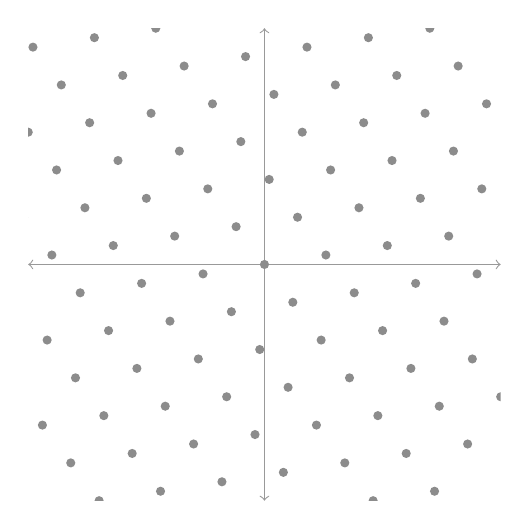
\begin{tikzpicture}

  \begin{scope}[scale=.6]
    \coordinate (Origin)   at (0,0);
    \coordinate (XAxisMin) at (-5,0);
    \coordinate (XAxisMax) at (5,0);
    \coordinate (YAxisMin) at (0,-5);
    \coordinate (YAxisMax) at (0,5);
    \draw [thin, black!40, <->] (XAxisMin) -- (XAxisMax);% Draw x axis
    \draw [thin, black!40,<->] (YAxisMin) -- (YAxisMax);% Draw y axis
    %\draw[style=help lines,dashed,black!20] (-5,-5) grid[step=1cm] (5,5);

    \begin{scope}
      \clip (-5,-5) rectangle (5,5); % Clips the picture...
      \pgftransformcm{1}{0.6}{0.7}{1}{\pgfpoint{0cm}{0cm}}

      % setup the nodes
      \foreach \x in {-15,...,15}
      \foreach \y in {-15,...,15}
      {
        \node[shape=circle,fill=black!45,scale=0.35] (\x-\y) at (2*\x,\y+3){};
      }
    \end{scope}
  \end{scope}

\end{tikzpicture}
\tikzset{external/export=false}

\tiny Picture credit: David Wong
\end{column}
\end{columns}
\end{frame}

\begin{frame}[label={sec:org654d7ef},fragile]{Shortest Vector Problem}
\begin{columns}
\begin{column}{0.5\columnwidth}
\begin{definition}
Given a lattice basis \(\mat{B}\), find a shortest non-zero vector in \(\Lambda(\mat{B})\).
\end{definition}

\begin{itemize}
\item The most natural problem on lattices
\item We write \(\lambda_{1}(\Lambda)\) for the Euclidean norm of a shortest vector.
\item NP-hard to solve exactly
\item Cryptography relies on approximate variants without such a reduction
\end{itemize}
\end{column}

\begin{column}{0.5\columnwidth}
\tikzset{external/export=true}
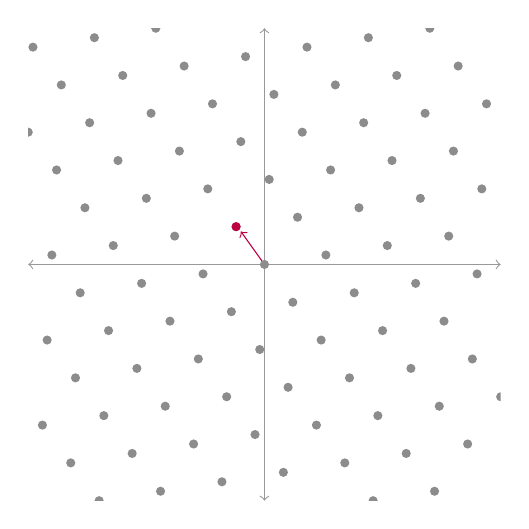
\begin{tikzpicture}
  \begin{scope}[scale=.6]
    \coordinate (Origin)   at (0,0);
    \coordinate (XAxisMin) at (-5,0);
    \coordinate (XAxisMax) at (5,0);
    \coordinate (YAxisMin) at (0,-5);
    \coordinate (YAxisMax) at (0,5);
    \draw [thin, black!40, <->] (XAxisMin) -- (XAxisMax);% Draw x axis
    \draw [thin, black!40,<->] (YAxisMin) -- (YAxisMax);% Draw y axis
    \draw [thin, purple,->] (0,0) -- (-.5,.7);
    % \draw[style=help lines,dashed,black!20] (-5,-5) grid[step=1cm] (5,5);

    \begin{scope}
      \clip (-5,-5) rectangle (5,5); % Clips the picture...
      \pgftransformcm{1}{0.6}{0.7}{1}{\pgfpoint{0cm}{0cm}}

      % setup the nodes
      \foreach \x in {-15,...,15}
      \foreach \y in {-15,...,15}
      {
        \node[shape=circle,fill=black!45,scale=0.35] (\x-\y) at (2*\x,\y+3){};
      }
    \end{scope}
    % our little node
    \node[shape=circle,fill=purple,scale=0.35] at (-.6,.8){};
  \end{scope}

\end{tikzpicture}
\tikzset{external/export=false}

\tiny Picture credit: David Wong
\end{column}
\end{columns}
\end{frame}

\begin{frame}[label={sec:org0e82673}]{Bounded Distance Decoding}
\begin{columns}
\begin{column}{0.5\columnwidth}
\begin{definition}
Given a lattice basis \(\mat{B}\), a vector \(\vec{t}\), and a parameter \(0 < \alpha\) such that the Euclidean distance \textnormal{dist}\((\vec{t},\vec{B}) < \alpha \cdot \lambda_{1}(\Lambda(\vec{B}))\), find the lattice vector \(\vec{v} \in \Lambda(\vec{B})\) which is closest to \(\vec{t}\).
\end{definition}

\begin{itemize}
\item When \(\alpha < 1/2\) unique decoding is guaranteed but for \(\alpha < 1\) we typically still expect unique decoding.
\item BDD is a special case of the Closest Vector Problem where there is no bound on the distance to the lattice.
\end{itemize}
\end{column}

\begin{column}{0.5\columnwidth}
\tikzset{external/export=true}
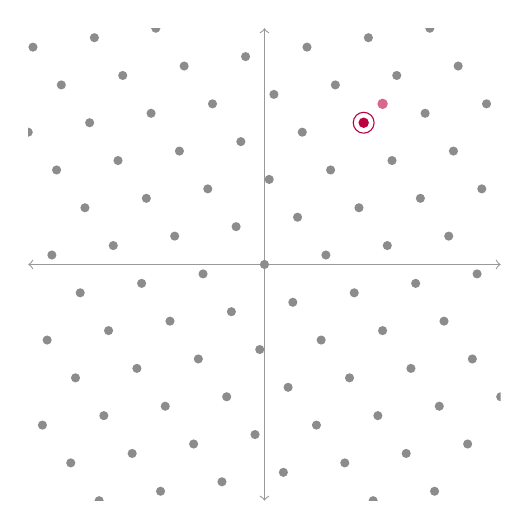
\begin{tikzpicture}

  \begin{scope}[scale=.6,shift={(12,0)}]
    \coordinate (Origin)   at (0,0);
    \coordinate (XAxisMin) at (-5,0);
    \coordinate (XAxisMax) at (5,0);
    \coordinate (YAxisMin) at (0,-5);
    \coordinate (YAxisMax) at (0,5);
    \draw [thin, black!40, <->] (XAxisMin) -- (XAxisMax);% Draw x axis
    \draw [thin, black!40,<->] (YAxisMin) -- (YAxisMax);% Draw y axis
    % \draw[style=help lines,dashed,black!20] (-5,-5) grid[step=1cm] (5,5);


    \begin{scope}
      \clip (-5,-5) rectangle (5,5); % Clips the picture...
      \pgftransformcm{1}{0.6}{0.7}{1}{\pgfpoint{0cm}{0cm}}

      % setup the nodes
      \foreach \x in {-15,...,15}
      \foreach \y in {-15,...,15}
      {
        \node[shape=circle,fill=black!45,scale=0.35] (\x-\y) at (2*\x,\y+3){};
      }
    \end{scope}

    % our little node
    \node[shape=circle,fill=purple!60,scale=0.4] at (2.5,3.4){};
    \node[shape=circle,fill=purple,scale=0.4] at (2.1,3){};
    \node[shape=circle,fill=none,draw=purple,scale=0.8] at (2.1,3){};

  \end{scope}

\end{tikzpicture}
\tikzset{external/export=false}

\tiny Picture credit: David Wong
\end{column}
\end{columns}
\end{frame}

\begin{frame}[label={sec:org24759e7}]{LWE \textbf{is} Bounded Distance Decoding (BDD) on Random \(q\)-ary Lattices}
Let
\[
\mat{L} =  \begin{pmatrix}
    q\mat{I} & \mat{A}\\
    0 & \mat{I}\\
  \end{pmatrix}
\]
We can reformulate the matrix form of the LWE equation \(\vec{A} \cdot \vec{s} + \vec{e} \equiv \vec{c} \bmod q\) as a linear system over the Integers as:
\[
  \mat{L} \cdot
  \begin{pmatrix}
    \vec{*}\\
    \vec{s}
  \end{pmatrix} +
  \begin{pmatrix}
    \vec{e}\\
    -\vec{s}
  \end{pmatrix}  
 = 
  \begin{pmatrix}
    q\mat{I} & -\mat{A}\\
    0 & \mat{I}\\
  \end{pmatrix} \cdot
  \begin{pmatrix}
    \vec{*}\\
    \vec{s}
  \end{pmatrix} +
  \begin{pmatrix}
    \vec{e}\\
    -\vec{s}
  \end{pmatrix}  
= 
  \begin{pmatrix}
    \vec{c}\\
    \vec{0}
  \end{pmatrix}
\]

The vector \((\vec{c}^T, \vec{0}^T)^T\) is close to the lattice \(\Lambda\left(\mat{L}\right)\) with offset \((\vec{e}^T, -\vec{s}^T)^T\).
\end{frame}


\begin{frame}[label={sec:org561cd12}]{Is that a Good Choice?}
\begin{itemize}
\item Maybe BDD on random \(q\)-ary lattices is easier than BDD in general?
\item Maybe BDD is easier than SVP?
\end{itemize}
\end{frame}

\begin{frame}[label={sec:org2ad245b}]{Sketch: BDD on Random \(q\)-ary Lattices solves BDD on any Lattice}
\begin{itemize}
\item We are given some basis \(\mat{B} \in \ZZ^{d \times d}\) and some target \(\vec{t}\) s.t. \(\vec{t} = \mat{B}\cdot \vec{s} + \vec{e}\) with \(\vec{e}\) small
\item Pick some large \(q \geq 2^{2d}\)
\item Sample some \(\mat{U}\) (see below)
\item Set \(\mat{A} = \mat{U}\cdot \mat{B} \bmod q\) and consider \(\vec{c} = \mat{U} \cdot \vec{t} + \vec{e}'\) with \({\vec{e}'}\) small
\begin{align*}
\vec{c} &= \mat{U} \cdot \vec{t} + \vec{e}' = \mat{U} \cdot \left(\mat{B}\cdot \vec{s} + \vec{e} \right) + \vec{e}' = \mat{U} \cdot \mat{B}\cdot \vec{s} + \mat{U} \cdot \vec{e} + \vec{e}' = \mat{A} \cdot \vec{s} + \vec{e}''
\end{align*}
\item We can pick \(\mat{U}\)
\begin{itemize}
\item large enough to make \(\mat{A}\) uniform mod \(q\) and
\item small enough to make \(\mat{U} \cdot \vec{e} + \vec{e}'\) small and well distributed
\end{itemize}
using "smoothing parameter" arguments on \(\Lambda(\mat{B}^{-T})\)
\end{itemize}

\fullcite{Regev:2009:LLE}
\end{frame}



\begin{frame}[label={sec:org63ea9b0}]{Sketch: Solving BDD on any Lattice implies solving GapSVP}
Say we want to decide if \(\lambda_{1}(\Lambda) \leq 1\) or \(\lambda_{1}(\Lambda) > \gamma\) and we have a BDD solver with \(\alpha = c\cdot \gamma\).

\begin{itemize}
\item Pick a random \(\vec{z} \in \Lambda\), add a small error \(\vec{e}\) of norm \(c\cdot \gamma\)
\item Run the BDD solver.
\item If it returns \(\vec{z}\) then output \(\lambda_{1}(\Lambda) > \gamma\), else output \(\lambda_{1}(\Lambda) \leq 1\).
\end{itemize}

\fullcite{STOC:Peikert09}

\begin{block}{}
Regev showed: If you have a BDD solver you can find a short basis on a quantum computer

\fullcite{Regev:2009:LLE}
\end{block}
\end{frame}

\begin{frame}[label={sec:org9e04fca},fragile]{Concrete Hardness: Cryptanalysis}
 \begin{itemize}
\item This tells us random \(q\)-ary lattices are not a terrible choice
\item To establish how long it actually takes to solve LWE, we rely on cryptanalysis
\lstset{language=sage,label= ,caption= ,captionpos=b,numbers=none}
\begin{lstlisting}
load("estimator.py")
primal_usvp(n=768, q=2^13, alpha=2^-11, reduction_cost_model=BKZ.ADPS16)
\end{lstlisting}
(rop: 2\textsuperscript{183.4}, red: 2\textsuperscript{183.4}, delta\textsubscript{0}: 1.002888, beta:  628, d: 1504, m: 735)
\end{itemize}

\fullcite{JMC:AlbPlaSco15}
\end{frame}

\section{Variants}
\label{sec:org1a931be}

\begin{frame}[label={sec:org0d2267d}]{LWE}
\[
\begin{pmatrix}c_{0} \\ c_{1} \\ c_{2} \\ c_{3} \\ c_{4} \\ c_{5} \\ c_{6} \\ c_{7}\end{pmatrix} = 
\begin{pmatrix}
a_{0,0} & a_{0,1} & a_{0,2} & a_{0,3} & a_{0,4} & a_{0,5} & a_{0,6} & a_{0,7}\\
a_{1,0} & a_{1,1} & a_{1,2} & a_{1,3} & a_{1,4} & a_{1,5} & a_{1,6} & a_{1,7}\\
a_{2,0} & a_{2,1} & a_{2,2} & a_{2,3} & a_{2,4} & a_{2,5} & a_{2,6} & a_{2,7}\\
a_{3,0} & a_{3,1} & a_{3,2} & a_{3,3} & a_{3,4} & a_{3,5} & a_{3,6} & a_{3,7}\\
a_{4,0} & a_{4,1} & a_{4,2} & a_{4,3} & a_{4,4} & a_{4,5} & a_{4,6} & a_{4,7}\\
a_{5,0} & a_{5,1} & a_{5,2} & a_{5,3} & a_{5,4} & a_{5,5} & a_{5,6} & a_{5,7}\\
a_{6,0} & a_{6,1} & a_{6,2} & a_{6,3} & a_{6,4} & a_{6,5} & a_{6,6} & a_{6,7}\\
a_{7,0} & a_{7,1} & a_{7,2} & a_{7,3} & a_{7,4} & a_{7,5} & a_{7,6} & a_{7,7}\\
\end{pmatrix} \cdot
\begin{pmatrix}s_{0} \\ s_{1} \\ s_{2} \\ s_{3} \\ s_{4} \\ s_{5} \\ s_{6} \\ s_{7}\end{pmatrix} +
\begin{pmatrix}e_{0} \\ e_{1} \\ e_{2} \\ e_{3} \\ e_{4} \\ e_{5} \\ e_{6} \\ e_{7}\end{pmatrix}
\]

\begin{block}{Performance}
Storage: \(\mathcal{O}(n^{2})\); Computation \(\mathcal{O}(n^{2})\)
\end{block}
\end{frame}

\begin{frame}[label={sec:orgb52b381}]{Ring-LWE/Polynomial-LWE}
\[
\begin{pmatrix}c_{0} \\ c_{1} \\ c_{2} \\ c_{3} \\ c_{4} \\ c_{5} \\ c_{6} \\ c_{7}\end{pmatrix} = 
\begin{pmatrix}
\alert{a_{0}} & -a_{7} & -a_{6} & -a_{5} & -a_{4} & -a_{3} & -a_{2} & -a_{1} \\
\alert{a_{1}} & a_{0} & -a_{7} & -a_{6} & -a_{5} & -a_{4} & -a_{3} & -a_{2} \\
\alert{a_{2}} & a_{1} & a_{0} & -a_{7} & -a_{6} & -a_{5} & -a_{4} & -a_{3} \\
\alert{a_{3}} & a_{2} & a_{1} & a_{0} & -a_{7} & -a_{6} & -a_{5} & -a_{4} \\
\alert{a_{4}} & a_{3} & a_{2} & a_{1} & a_{0} & -a_{7} & -a_{6} & -a_{5} \\
\alert{a_{5}} & a_{4} & a_{3} & a_{2} & a_{1} & a_{0} & -a_{7} & -a_{6} \\
\alert{a_{6}} & a_{5} & a_{4} & a_{3} & a_{2} & a_{1} & a_{0} & -a_{7} \\
\alert{a_{7}} & a_{6} & a_{5} & a_{4} & a_{3} & a_{2} & a_{1} & a_{0}
\end{pmatrix}\cdot
\begin{pmatrix}s_{0} \\ s_{1} \\ s_{2} \\ s_{3} \\ s_{4} \\ s_{5} \\ s_{6} \\ s_{7}\end{pmatrix} +
\begin{pmatrix}e_{0} \\ e_{1} \\ e_{2} \\ e_{3} \\ e_{4} \\ e_{5} \\ e_{6} \\ e_{7}\end{pmatrix}
\]
\end{frame}

\begin{frame}[label={sec:orgdb6cc74}]{Ring-LWE/Polynomial-LWE}
\begin{align*}
\sum_{i=0}^{n-1} c_{i} \cdot X^{i} &= \left(\sum_{i=0}^{n-1} a_{i} \cdot X^{i}\right) \cdot \left(\sum_{i=0}^{n-1} s_{i} \cdot X^{i}\right) + \sum_{i=0}^{8} e_{i} \cdot X^{i} \bmod X^{n} +1\\
c(X) &= a(X) \cdot s(X) + e(X) \bmod \phi(X)
\end{align*}

\begin{block}{Performance (\(n\) is a power of two)}
Storage: \(\mathcal{O}(n)\); Computation \(\mathcal{O}(n \log n)\)
\end{block}

\fullcite{EC:LyuPeiReg10}
\end{frame}

\begin{frame}[label={sec:org27a709f}]{Module-LWE}
\[
\begin{pmatrix}c_{0,0} \\ c_{0,1} \\ c_{0,2} \\ c_{0,3} \\ c_{1,0} \\ c_{1,1} \\ c_{1,2} \\ c_{1,3}\end{pmatrix} = 
\left(\begin{array}{rrrr|rrrr}
\alert{a_{0,0}} & -a_{0,3} & -a_{0,2} & -a_{0,1} & \alert{a_{1,0}} & -a_{1,3} & -a_{1,2} & -a_{1,1} \\
\alert{a_{0,1}} &  a_{0,0} & -a_{0,3} & -a_{0,2} & \alert{a_{1,1}} &  a_{1,0} & -a_{1,3} & -a_{1,2} \\
\alert{a_{0,2}} &  a_{0,1} &  a_{0,0} & -a_{0,3} & \alert{a_{1,2}} &  a_{1,1} &  a_{1,0} & -a_{1,3} \\
\alert{a_{0,3}} &  a_{0,2} &  a_{0,1} &  a_{0,0} & \alert{a_{1,3}} &  a_{1,2} &  a_{1,1} &  a_{1,0} \\
\hline
\alert{a_{2,0}} & -a_{2,3} & -a_{2,2} & -a_{2,1} & \alert{a_{3,0}} & -a_{3,3} & -a_{3,2} & -a_{3,1} \\
\alert{a_{2,1}} &  a_{2,0} & -a_{2,3} & -a_{2,2} & \alert{a_{3,1}} &  a_{3,0} & -a_{3,3} & -a_{3,2} \\
\alert{a_{2,2}} &  a_{2,1} &  a_{2,0} & -a_{2,3} & \alert{a_{3,2}} &  a_{3,1} &  a_{3,0} & -a_{3,3} \\
\alert{a_{2,3}} &  a_{2,2} &  a_{2,1} &  a_{2,0} & \alert{a_{3,3}} &  a_{3,2} &  a_{3,1} &  a_{3,0} \\
\end{array}\right)\cdot
\begin{pmatrix}s_{0} \\ s_{1} \\ s_{2} \\ s_{3} \\ s_{4} \\ s_{5} \\ s_{6} \\ s_{7}\end{pmatrix} +
\begin{pmatrix}e_{0} \\ e_{1} \\ e_{2} \\ e_{3} \\ e_{4} \\ e_{5} \\ e_{6} \\ e_{7}\end{pmatrix}
\]
\end{frame}

\begin{frame}[label={sec:orga25f397}]{Module-LWE}
\[
\begin{pmatrix} c_{0}(X) \\ c_{1}(X) \end{pmatrix} =
\begin{pmatrix} a_{0}(X) & a_{1}(X) \\ a_{2}(X) & a_{3}(X) \end{pmatrix} \cdot
\begin{pmatrix} s_{0}(X) \\ s_{1}(X) \end{pmatrix} +
\begin{pmatrix} e_{0}(X) \\ e_{1}(X) \end{pmatrix}
\]

\begin{block}{Performance (\(n\) is a power of two)}
Storage: \(\mathcal{O}(k^{2} \cdot n)\); Computation \(\mathcal{O}(k^{2} \cdot n \log n)\)
\end{block}
\fullcite{Langlois:2015:WCA}
\end{frame}

\begin{frame}[label={sec:org521db13}]{LWR}
Instead of "wiping" the lower-order bits of \(\vec{c}_{i} = \mat{A} \cdot \vec{s}\) by adding \(\vec{e}_{i}\), throw them away
\begin{itemize}
\item More formally, output \[ \left\lfloor{\frac{p}{q} \cdot  (\mat{A} \cdot \vec{s})} \right\rceil \]  for some \(p < q\).
\item This is no easier than LWE if  \[ \left\lfloor{\frac{p}{q} \cdot  (\mat{A} \cdot \vec{s})} \right\rceil =    \left\lfloor{\frac{p}{q} \cdot  (\mat{A} \cdot \vec{s} + \vec{e})} \right\rceil  \]
\item Can be quite fast if \(p,q\) are powers of two, saves bandwidth
\end{itemize}

\fullcite{EC:BanPeiRos12}  
\end{frame}

\section{LWE Encryption}
\label{sec:orgefbe771}

\begin{frame}[label={sec:org79b5b8e}]{Convention}
\begin{itemize}
\item I am going to use the Ring-LWE formulation \[c_{i}(X) = a_{i}(X)\cdot s(X) + e_{i}(X)\]
Thus, each sample corresponds to "\(n\) LWE samples"
\item I will suppress the "\((X)\)" in "\(a(X)\)" etc.
\item I will assume \(s\) is "small" and that the product of two "small" things is "small".
\item I will write \(\alert{e_{i}}\) to emphasise that \(e_{i}\) is small.
\end{itemize}

\begin{block}{TL;DR: I will write}
\[c_{i} = a_{i}\cdot \alert{s} + \alert{e_{i}}\]
\end{block}
\end{frame}

\begin{frame}[label={sec:org58e405b}]{DH to Ring-LWE Dictionary}
\begin{center}
\begin{tabular}{ll}
DH Land & Ring-LWE Land\\
\hline
\(g\) & \(a\)\\
\(g^x\) & \(a\cdot {s} + \alert{e}\)\\
 & \\
\(g^x \cdot g^y = g^{x+y}\) & \((a\cdot {s} + \alert{e_0}) + (a \cdot {t} + \alert{e_1}) = a \cdot {(s+t)} + \alert{e'}\)\\
 & \\
\((g^a)^b = (g^b)^a\) & \((a\cdot \alert{s} + \alert{e})\cdot \alert{t} = (a\cdot \alert{s} \cdot \alert{t} + \alert{e} \cdot \alert{t})\)\\
 & \(\approx a\cdot \alert{s} \cdot \alert{t} \approx (a\cdot \alert{t} + \alert{e})\cdot \alert{s}\)\\
 & \\
\((g, g^a, g^b, g^{ab})\) & \((a,\ a\cdot \alert{s} + \alert{e},\ a\cdot \alert{t} + \alert{d},\ a \cdot \alert{s} \cdot \alert{t} + \alert{e'})\)\\
\(\approx_c (g, g^a, g^b, u)\) & \(\approx_c (a,\ a\cdot \alert{s} + \alert{e},\ a\cdot \alert{t} + \alert{d},\ u)\)\\
\end{tabular}

\end{center}
\end{frame}


\begin{frame}[label={sec:org3f1e679}]{Regev}
You have already seen it.

\begin{description}
\item[{KeyGen}] Publish \(c_{i} = a_{i} \cdot s + \alert{e_{i}}\) for \(i=0,\ldots, \lceil 2\, n \log q\rceil\)
\item[{Encrypt}] \[d_{0} = \sum \alert{b_{i}} \cdot a_{i},\quad  d_{1} = \left(\sum \alert{b_{i}} \cdot c_{i} \right) + q/2 \cdot m  \textnormal{ with } \alert{b_{i}} \in \bin, m \in \bin^{n}\]
\item[{Decrypt}] \begin{align*}
\left\lfloor \frac{2}{q} \cdot \left(d_{1} - d_{0} \cdot s\right) \right\rceil &= \left\lfloor \frac{2}{q} \cdot \left(\left(\sum \alert{b_{i}} \cdot c_{i} \right) + \frac{q}{2} \cdot m - \sum \alert{b_{i}} \cdot a_{i} \cdot s\right) \right\rceil\\
&= \left\lfloor \frac{2}{q} \cdot \left(\left(\sum \alert{b_{i}} \cdot (a_{i} \cdot s + \alert{e_{i}}) \right) + \frac{q}{2} \cdot m - \sum \alert{b_{i}} \cdot a_{i} \cdot s\right) \right\rceil\\
&= \left\lfloor \frac{2}{q} \cdot \left(\left(\sum \alert{b_{i} \cdot e_{i}} \right) + \frac{q}{2} \cdot m \right) \right\rceil = m
\end{align*}
\end{description}

The public key is indistinguishable from uniform by the LWE assumption and \(\sum b_{i} \cdot a_{i}\) is statistically close to uniformly random by the Leftover Hash Lemma (LHL).
\end{frame}

\begin{frame}[label={sec:org2c3980b}]{ElGamal \& LPR10}
\textbf{ElGamal}

\begin{description}
\item[{KeyGen}] \(h = g^{x}\)
\item[{Encrypt}] \(d_{0},\ d_{1} = \left({g^{r},\  m \cdot h^{r}}\right)\) for some random \(r\)
\item[{Decrypt}] \(d_{1} / d_{0}^{x} = m \cdot (g^{x})^{r} / (g^{r})^{x} = m\)
\end{description}

\textbf{\cite{EC:LyuPeiReg10}}\footnote{\textbf{All} NIST PQC candidates based on (Ring-/Module-)LWE encrypt like this}

\begin{description}
\item[{KeyGen}] \(c = a \cdot \alert{s} + \alert{e}\)
\item[{Encrypt}] \(d_{0}, \ d_{1} = \alert{v} \cdot a + \alert{e'},\ \alert{v} \cdot c + \alert{e''} + q/2 \cdot m\)
\item[{Decrypt}] \begin{align*}
\left\lfloor \frac{2}{q} \cdot \left(d_{1} - d_{0} \cdot \alert{s}\right) \right\rceil &= \left\lfloor \frac{2}{q} \cdot \left({\alert{v} \cdot (a \cdot \alert{s} + \alert{e}) + \alert{e''} + \frac{q}{2} \cdot m - \left(\alert{v} \cdot a + \alert{e'}\right) \cdot \alert{s}}\right) \right\rceil\\
&= \left\lfloor \frac{2}{q} \cdot \left({\alert{v} \cdot \alert{e} + \alert{e''} + \frac{q}{2} \cdot m - \alert{e'} \cdot \alert{s}}\right) \right\rceil = m\\
\end{align*}
\end{description}
\end{frame}


\begin{frame}[label={sec:org1158524}]{Proof Sketch}
\begin{description}
\item[{KeyGen}] \(c = a \cdot \alert{s} + \alert{e}\)
\begin{itemize}
\item The public key \((a,c)\) is indistinguishable from uniform \((u', u'')\) by the (Ring-)LWE assumption
\end{itemize}

\item[{Encrypt}] \(d_{0}, \ d_{1} = \alert{v} \cdot a + \alert{e'},\ \alert{v} \cdot c + \alert{e''} + q/2 \cdot m\)
\begin{itemize}
\item Then \(\alert{v} \cdot u' + \alert{e''},\ \alert{v} \cdot u'' + \alert{e''}\) is indistinguishable from uniform by the (Ring)-LWE assumption
\end{itemize}
\end{description}
\end{frame}

\begin{frame}[allowframebreaks]{Reconciliation}
Once you have ElGamal, recovering Diffie-Hellman is straight forward.

\begin{description}
\item[{Common}] \(a\)
\item[{Alice}] \(c_{0} = \alert{s} \cdot a + \alert{e_{0}}\)
\item[{Bob}] \(c_{1} = a \cdot \alert{t} + \alert{e_{1}}\)
\item[{Shared}] \[c_{0} \cdot \alert{t} = ( \alert{s} \cdot a + \alert{e_{0}})\cdot \alert{t} \approx \alert{s} \cdot a \cdot \alert{t} \approx \alert{s} \cdot (a \cdot \alert{t} + \alert{e_{1}}) = \alert{s} \cdot c_{1} \]
\end{description}

\framebreak

\[c_{0} \cdot \alert{t} = ( \alert{s} \cdot a + \alert{e_{0}})\cdot \alert{t} \approx \alert{s} \cdot a \cdot \alert{t} \approx \alert{s} \cdot (a \cdot \alert{t} + \alert{e_{1}}) = \alert{s} \cdot c_{1} \]

\begin{itemize}
\item The problem with this construction is that "\(\approx\)" \(\neq\) "\(=\)"
\item Need to send a "hint" how to round correctly (2nd most significant bit) \footfullcite{EPRINT:DinXieLin12}
\item Cannot have efficient Non-interactive Key Exchange (NIKE) without new ideas
\item Here be {\color{lightgray}{dragons} }patents
\item NIST asked for "key exchange" but meant "key encapsulation", can build former generically from latter
\end{itemize}
\end{frame}


\section{CCA Security}
\label{sec:org04774de}

\begin{frame}[label={sec:org66e23b3}]{Active Attacks}
\begin{itemize}
\item Recall decryption
\[\left\lfloor \frac{2}{q} \cdot \left(d_{1} - d_{0} \cdot {s}\right) \right\rceil = \left\lfloor \frac{2}{q} \cdot \left({\frac{q}{2} \cdot m + {v} \cdot {e} - {e'} \cdot {s} + {e''}}\right) \right\rceil = m\]
\item When the result of the rounding \(\neq m\) this contains information about
\[{v} \cdot {e} - {e'} \cdot {s} + {e''}\]
where the attacker/encrypter controls \(v, e'', e'\) and would like to learn \(s,e\).
\end{itemize}
\end{frame}

\begin{frame}[label={sec:orge5f8678}]{FO Transform (KEM Variant)}
\begin{description}
\item[{Encrypt}] \(v,e', e'' \gets \operatorname{H}(\mathsf{seed})\) and \(m = \mathsf{seed}\) for some hash function \(\operatorname{H}\).
\item[{Decrypt}] After decryption
\begin{itemize}
\item compute \(v,e', e'' \gets \operatorname{H}(m')\) and
\item check \(c_{0} \overset{?}{=} v\cdot a + e'\) and \(c_{1} \overset{?}{=} v \cdot c + e'' + q/2 \cdot m'\).
\end{itemize}
\end{description}

\fullcite{JC:FujOka13}

\fullcite{TCC:HofHovKil17}  
\end{frame}

\begin{frame}[label={sec:orga7beb36}]{(Q)ROM}
\begin{itemize}
\item The FO transform was originally proven secure when modelling the hash function as a Random Oracle (RO)
\item Hash functions are public functions and thus can be implemented on a quantum computer
\item We must model the hash function as a Quantum Random Oracle (QRO), accepting superposition queries
\end{itemize}

\fullcite{EC:SaiXagYam18}
\end{frame}

\section{Practical Performance}
\label{sec:orge44c465}

\begin{frame}[label={sec:org95c8c25}]{Baseline: Pre Quantum Cryptography}
\begin{columns}[t]
\begin{column}{0.5\columnwidth}
\textbf{RSA 2048}

\begin{center}
\begin{tabular}{lr}
Key generation & \(\approx\) 130,000,000 cycles\\
Encapsulation & \(\approx\) 20,000 cycles\\
Decapsulation & \(\approx\) 2,700,000 cycles\\
Ciphertext & 256 bytes\\
Public key & 256 bytes\\
\end{tabular}

\end{center}

\small \url{https://bench.cr.yp.to/results-kem.html}
\end{column}

\begin{column}{0.5\columnwidth}
\textbf{Curve25519}

\begin{center}
\begin{tabular}{lr}
Key generation & \(\approx\) 60,000 cycles\\
Key agreement & \(\approx\) 160,000 cycles\\
 & \\
Public key & 32 bytes\\
Key Share & 32 bytes\\
\end{tabular}

\end{center}

\small \url{https://eprint.iacr.org/2015/943}
\end{column}
\end{columns}
\end{frame}


\begin{frame}[label={sec:orga47d8d6}]{Kyber}
\begin{columns}[t]
\begin{column}{0.5\columnwidth}
\textbf{Curve25519}

\begin{center}
\begin{tabular}{lr}
Key generation & \(\approx\) 60,000 cycles\\
Key agreement & \(\approx\) 160,000 cycles\\
 & \\
Public key & 32 bytes\\
Key Share & 32 bytes\\
\end{tabular}

\end{center}

\small \url{https://eprint.iacr.org/2015/943}
\end{column}

\begin{column}{0.5\columnwidth}
\textbf{Kyber-768 NIST PQC Round 2 submission:}

\begin{center}
\begin{tabular}{lr}
Key generation & \(\approx\)  42,000 cycles\\
Encapsulation & \(\approx\)  60,000 cycles\\
Decapsulation & \(\approx\)  52,000 cycles\\
Ciphertext & 1,088 bytes\\
Public key & 1,184 bytes\\
\end{tabular}

\end{center}

\small \url{https://bench.cr.yp.to/results-kem.html}
\end{column}
\end{columns}

\begin{block}{Interpretation}
\begin{itemize}
\item An Ethernet frame takes 1,500 bytes
\item Your laptop does about \(2\cdot 10^{9}\) cycles per second
\end{itemize}
\end{block}
\end{frame}

\begin{frame}[label={sec:org70e71b1},standout]{Fin}
\begin{center}
\Huge \alert{Thank You}
\end{center}
\end{frame}

\begin{frame}[allowframebreaks]{References}
\renewcommand*{\bibfont}{\scriptsize}
\printbibliography[heading=none]
\end{frame}
\end{document}